\documentclass{article}

% Official NeurIPS 2026 single-blind workshop format.
\usepackage[sglblindworkshop]{neurips_2026}
\workshoptitle{Interpreting Agent Behavior}

\usepackage[utf8]{inputenc}
\usepackage[T1]{fontenc}
\usepackage{hyperref}
\hypersetup{hidelinks}
\usepackage{url}
\usepackage{booktabs}
\usepackage{amsmath}
\usepackage{amsfonts}
\usepackage{microtype}
\usepackage{xspace}
\usepackage{xcolor}
\usepackage{tabularx}
\usepackage{array}
\usepackage{tikz}
\usetikzlibrary{arrows.meta,positioning}

\newcommand{\systemname}{\textsc{RankSmith}\xspace}
\newcommand{\pct}{\%}
\newcolumntype{Y}{>{\raggedright\arraybackslash}X}

\title{Winning the Percentile, Not the Payoff:\\
A Deterministic, Experiment-Driven Agent for GLEE}

\author{%
  Author Name \thanks{Author details are intentionally left as a draft placeholder.}\\
  Affiliation \\
  \texttt{email@example.com}
}

\begin{document}

\maketitle

\begin{abstract}
GLEE evaluates agents in bargaining, bilateral negotiation, and repeated persuasion, but its competition objective is not expected payoff: each outcome is ranked against payoffs from the exact configuration and role before entering an opponent-adjusted rating. We present \systemname, a deterministic, LLM-free agent built from game-theoretic structure, empirical field models, and a safety layer that makes every decision total and auditable. The main lesson from development is methodological. Several apparently strong changes vanished or reversed after retaining all assigned outcomes, defining cohorts before treatment, checking that a flag changed the submitted action, and auditing the final action sent to the server. At a protected August 26 snapshot, our best agent had an overall displayed rating of 2562, with family ratings 2542/2732/2413 for bargaining/negotiation/persuasion. We describe the agent, report structural findings from live behavior, and show how rank-aware experimentation prevented selection bias and invalid replay assumptions from becoming policy.
\end{abstract}

\section{Introduction}

GLEE standardizes two-player language-based economic games spanning alternating-offer bargaining, bilateral trade, and Bayesian persuasion \citep{shapira2024glee}. The live competition adds a distinctive objective: a payoff $y$ is converted to an empirical percentile $q=F_{c,r}(y)$ within the exact configuration $c$ and role $r$, adjusted for opponent strength, and mapped to a per-game rating
\begin{equation}
G=2000+8000(q-0.5), \qquad \Delta R=\eta(G-R),
\label{eq:rating}
\end{equation}
with a decaying step size $\eta$ \citep{gleecompetition2026}. Consequently, an outcome that maximizes dollars need not maximize rank. A zero can be median in a structurally infeasible cell but bottom-decile in a cell where others trade; moving just above an atom in the payoff distribution can be worth more than a much larger dollar improvement elsewhere.

We built \systemname around this distinction. The online policy is deliberately conventional: exact or finite-horizon game-theoretic structure where available, conservative empirical floors where the field violates equilibrium, and deterministic posterior updates under hidden information. The less conventional contribution is the development loop. Every proposed change was treated as a falsifiable mechanism with a recoverable assignment, an all-outcome intent-to-treat cohort, and a wire-level audit. This mattered because the largest apparent gains were often measurement failures rather than strategy gains.

Our contributions are: (i) a deterministic, LLM-free agent covering all three GLEE families; (ii) structural live-field measurements that localize where performance is and is not recoverable; and (iii) an agent-behavior analysis protocol that detects treatment leakage, unreachable gates, survivorship bias, and fabricated outcomes before deployment.

\begin{figure}[t]
\centering
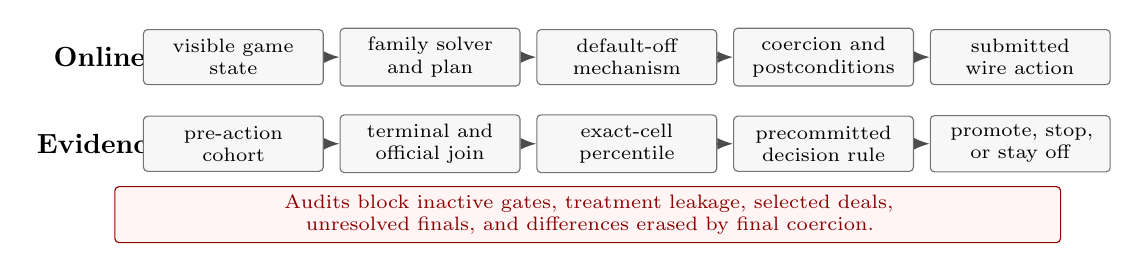
\begin{tikzpicture}[
  font=\scriptsize,
  box/.style={draw=black!55, rounded corners=1.5pt, align=center,
              minimum height=7mm, text width=2.05cm, fill=black!3},
  arr/.style={-{Latex[length=2mm]}, semithick, draw=black!70},
  warn/.style={draw=red!60!black, rounded corners=1.5pt, align=center,
               fill=red!4, text=red!55!black, inner sep=3pt}
]
\node[font=\bfseries] at (-1.0,0.75) {Online};
\node[box] (state) at (0.7,0.75) {visible game\\state};
\node[box, right=2mm of state] (solver) {family solver\\and plan};
\node[box, right=2mm of solver] (flag) {default-off\\mechanism};
\node[box, right=2mm of flag] (coerce) {coercion and\\postconditions};
\node[box, right=2mm of coerce] (wire) {submitted\\wire action};
\draw[arr] (state) -- (solver);
\draw[arr] (solver) -- (flag);
\draw[arr] (flag) -- (coerce);
\draw[arr] (coerce) -- (wire);

\node[font=\bfseries] at (-1.0,-0.35) {Evidence};
\node[box] (cohort) at (0.7,-0.35) {pre-action\\cohort};
\node[box, right=2mm of cohort] (join) {terminal and\\official join};
\node[box, right=2mm of join] (cdf) {exact-cell\\percentile};
\node[box, right=2mm of cdf] (rule) {precommitted\\decision rule};
\node[box, right=2mm of rule] (deploy) {promote, stop,\\or stay off};
\draw[arr] (cohort) -- (join);
\draw[arr] (join) -- (cdf);
\draw[arr] (cdf) -- (rule);
\draw[arr] (rule) -- (deploy);

\node[warn, text width=11.8cm] at (5.2,-1.25)
{Audits block inactive gates, treatment leakage, selected deals, unresolved finals, and differences erased by final coercion.};
\end{tikzpicture}
\caption{The action path and evidence path are both audited. A mechanism is not considered tested unless it reaches eligible states, fires, changes the final wire, and is evaluated on a cohort defined before that change.}
\label{fig:pipeline}
\end{figure}

\section{Agent design}

\paragraph{Total deterministic dispatcher.}
A single dispatcher selects a family policy, records its numerical plan and fired gates, coerces the result into the server schema, and applies final postconditions. Any exception degrades to a legal family-specific fallback instead of allowing a turn timeout. The submitted action, rather than an intermediate plan, is the unit audited in replay. The final protected agent used no neural model or LLM in its decision or message path.

\paragraph{Bargaining.}
For $k$ rounds remaining, the proposer share follows the finite recursion $f(1)=1$ and $f(k)=1-\delta_{\mathrm{resp}}f(k-1)$, approaching the Rubinstein solution under an infinite horizon \citep{rubinstein1982}. The agent blends this value with the field's strong 50/50 anchor, floors offers at a level the field actually accepts, and estimates continuation from the opponent's observed concession trail. A role audit over 4,001 games found a severe initial asymmetry (Alice 71.5th percentile, Bob 28.8th); an accept-floor correction made Bob the stronger seat in a later 500-game export.

\paragraph{Negotiation.}
With both values visible, the agent computes the zone of possible agreement (ZOPA) exactly and follows an interior reservation path. With values hidden, it uses role-specific anchors, Boulware concession, table-based acceptance, support bounds from the public value grid, and terminal rules. Structural inspection showed that all 6 complete-information value cells are feasible, while only 6 of 16 hidden-information cells are; thus 10 of 22 grid cells are infeasible. This prevents treating every no-deal as a policy failure.

\paragraph{Persuasion.}
The seller conditions recommendations on quality, prior expected value, and observed demand. The buyer maintains a discrete posterior over seller low-quality recommendation rates $q\in\{0,.125,.25,.5,.75,1\}$, updates it from the full recommendation stream, and purchases when posterior expected utility clears price. This is an adaptive analogue of the sender-receiver structure in Bayesian persuasion \citep{kamenica2011bayesian}. Text is parsed into positive, negative, or abstaining evidence; explicit declines are hard vetoes in the final policy.

\section{Rank-aware development and evaluation}

Figure~\ref{fig:pipeline} summarizes the contract used for uncertain changes. Behavioral changes landed default-off. When randomization was authorized, a stable hash of game ID assigned treatment per game; assignment occurred after eligibility was defined and was kept out of unrelated decision variables. Otherwise, we used a frozen named challenger and reported the comparison as observational.

The primary cohort was defined at the first structurally eligible pre-action turn and retained agreements, no-deals, walks, invalids, timeouts, immediate accepts, and unresolved results. Missing finals remained unresolved and blocked promotion. The primary metric was authenticated official per-game rating delta when joinable; a checked-in exact-cell payoff CDF supplied a diagnostic percentile. We never promoted on completed deals alone.

Reachability was a separate requirement: every mechanism had to show positive counts for eligible states, firings, and changed wire actions under the intended live stack. We then re-ran the flag-off and flag-on paths and compared the post-coercion action. This catches a clean-looking null from a flag nested under a disabled parent, as well as an apparent treatment that an action sanitizer later erases.

\begin{table}[t]
\centering
\small
\caption{Selected live behavior measurements. Counts include the stated cohort rather than only favorable outcomes.}
\label{tab:behavior}
\begin{tabularx}{\linewidth}{@{}p{3.3cm}p{3.2cm}Y@{}}
\toprule
Question & Measurement & Design implication \\
\midrule
How much negotiation is feasible? & complete 6/6; hidden 6/16 value cells & Evaluate close rate against the feasible ceiling, not 100\pct. \\
Are we refusing good hidden offers? & 89 of 14,732 no-deal decision turns (0.6\pct) exposed a profitable offer & Most hidden no-deals arise before a mutually acceptable price reaches us. \\
What happens in one-round complete information? & 384/384 offers claiming $<0.9$ of span closed; 0/78 at $\geq1.05$ closed & A sharp last-move frontier exists, but it does not identify multi-round response. \\
Does generated wording help? & LLM wording converted 46.3\pct versus 55.3\pct for templates & Keep decisions and messages deterministic; do not assume linguistic variety is persuasive. \\
\bottomrule
\end{tabularx}
\end{table}

\section{Results: what survived and what did not}

Table~\ref{tab:snapshot} reports the protected Agent 5 snapshot. These values summarize the deployed full stack; they are not a causal estimate of any component, and the competition had not yet closed.

\begin{table}[h]
\centering
\small
\caption{Displayed ratings at the losslessly banked August 26 snapshot.}
\label{tab:snapshot}
\begin{tabular}{@{}lrrrr@{}}
\toprule
 & Bargaining & Negotiation & Persuasion & Overall \\
\midrule
Agent 5 & 2542 & 2732 & 2413 & 2562 \\
\bottomrule
\end{tabular}
\end{table}

The more transferable result is the number of attractive changes we rejected. A replay sweep suggested that leaving only 10\pct of visible negotiation surplus to the opponent gained $+0.0121$ diagnostic percentile across four runs. Audit showed that unseen aggressive asks were accepted by the clone by construction, response bins were too coarse, hidden-value tables were populated mainly by agreements, and one flag changed three distinct quantities. We rejected the entire result.

Likewise, accepting every profitable hidden offer first appeared to gain $+0.07138$ per exposed decision. That counterfactual treated every observed rejection as a zero. Replaying the actual later continuation reversed the result to $-0.06628$ (95\pct bootstrap CI $[-0.08183,-0.05096]$) per exposed decision and $-0.00614$ over the 4,050-game cohort. A leader-trajectory clone produced an encouraging early official lift of $+1.812$ rating/game on 45 games, but the fixed 91-game checkpoint fell to $+0.869$ with CI $[-0.78,2.52]$, raised no-deals by 6.14 points, and was negative on one host; it failed its frozen promotion gates.

Finally, an outcome reader once imputed old missing finals as 5th-percentile abandonments. The collector had actually stopped with 11,737 results outstanding. Treating these records as unresolved rather than losses changed which experiments were even readable. These failures explain why our final policy contains fewer experimental mechanisms than the number of promising development plots might suggest.

\section{Agent Behavior Analysis}

We define alignment operationally: the visible state should select the intended family plan; a gate should fire only in its documented scope; coercion should preserve the intended semantic action; and the wire should be attributable to exactly one mechanism. Every turn log therefore stores the state fingerprint, plan, ordered gate trace, source, and submitted action. Paired reachability checks establish that a mechanism can change behavior before any outcome analysis, while independent readers recompute assignment and expected wires rather than trusting logged treatment labels.

This process found behavioral mismatches that aggregate score could not. A parser bought messages containing ``Not recommended'' because the positive token matched first; the corrected strict decline gates are limited to current-message buyer decisions and can only change buy to pass. A surplus-share probe randomized an offer target before the action branch, unintentionally changing accept/reject decisions even on turns that sent no offer. The probe was disabled because its outcome could not identify the intended price-response mechanism. In another case, a replay candidate replaced the entire control flag set instead of overlaying one change, silently measuring two strategies rather than one parameter.

The final Agent 5 snapshot had all per-game A/B flags explicitly off and used deterministic templates. This does not prove semantic alignment for arbitrary language or opponents; it shows that the deployed policy matched its encoded design under the audited GLEE action interface.

\section{Limitations and conclusion}

The live field is nonstationary, opponents adapt, and identical code showed roughly $\pm125$ rating dispersion in persuasion over ten hours. Hidden opponent values are never revealed, so per-game feasibility and many rejected-offer counterfactuals are not identifiable from our logs. Several full-stack comparisons are observational because the operator later prohibited live randomization. Our text findings concern this parser-heavy competition population and do not establish that natural language is generally useless. The August 26 rating is a dated snapshot, not a final placement.

Within those limits, \systemname demonstrates a practical principle for economic agents: optimize the scored rank, but distrust every measured gain until the treatment changes the final action and every assigned outcome is retained. In this competition, the discipline to reject false wins was itself a competitive advantage.

\newpage
\bibliographystyle{plainnat}
\bibliography{references}

\newpage
\section*{NeurIPS Paper Checklist}

\begin{enumerate}

\item {\bf Claims}
    \item[] Question: Do the main claims made in the abstract and introduction accurately reflect the paper's contributions and scope?
    \item[] Answer: \answerYes{}
    \item[] Justification: The abstract and Section 1 state the agent, methodological contribution, dated performance snapshot, and non-causal scope; Sections 5--6 qualify the claims.

\item {\bf Limitations}
    \item[] Question: Does the paper discuss the limitations of the work performed by the authors?
    \item[] Answer: \answerYes{}
    \item[] Justification: Section 6 discusses nonstationarity, unidentified hidden values, observational comparisons, rating noise, language generality, and the non-final snapshot.

\item {\bf Theory assumptions and proofs}
    \item[] Question: For each theoretical result, does the paper provide the full set of assumptions and a complete (and correct) proof?
    \item[] Answer: \answerNA{}
    \item[] Justification: The paper introduces no new theorem. It cites standard bargaining and persuasion models and reports empirical competition behavior.

\item {\bf Experimental result reproducibility}
    \item[] Question: Does the paper fully disclose all the information needed to reproduce the main experimental results of the paper to the extent that it affects the main claims and/or conclusions of the paper (regardless of whether the code and data are provided or not)?
    \item[] Answer: \answerYes{}
    \item[] Justification: Sections 3--5 specify cohort timing, assignment, retained outcomes, metrics, reachability, wire audits, checkpoints, and uncertainty for the principal results; the accompanying repository contains the corresponding readers and tests.

\item {\bf Open access to data and code}
    \item[] Question: Does the paper provide open access to the data and code, with sufficient instructions to faithfully reproduce the main experimental results, as described in supplemental material?
    \item[] Answer: \answerYes{}
    \item[] Justification: The agent code, tests, frozen analysis artifacts, and reader scripts are included with the submission. Private competition transcripts are not redistributed beyond the access allowed by the competition.

\item {\bf Experimental setting/details}
    \item[] Question: Does the paper specify all the training and test details (e.g., data splits, hyperparameters, how they were chosen, type of optimizer) necessary to understand the results?
    \item[] Answer: \answerYes{}
    \item[] Justification: The agent has no training or optimizer. Sections 2--4 specify the policy, public grid structure, cohorts, assignments, checkpoints, and evaluation units used for the reported analyses.

\item {\bf Experiment statistical significance}
    \item[] Question: Does the paper report error bars suitably and correctly defined or other appropriate information about the statistical significance of the experiments?
    \item[] Answer: \answerYes{}
    \item[] Justification: Section 4 reports bootstrap or approximate 95\% intervals for the treatment comparisons used to support the main methodological claims, and labels descriptive measurements as such.

\item {\bf Experiments compute resources}
    \item[] Question: For each experiment, does the paper provide sufficient information on the computer resources (type of compute workers, memory, time of execution) needed to reproduce the experiments?
    \item[] Answer: \answerNo{}
    \item[] Justification: The agent and readers are CPU-only and require no accelerator, but wall-clock and memory totals were not isolated from continuous live competition operation. We therefore do not claim a complete compute accounting.

\item {\bf Code of ethics}
    \item[] Question: Does the research conducted in the paper conform, in every respect, with the NeurIPS Code of Ethics \url{https://neurips.cc/public/EthicsGuidelines}?
    \item[] Answer: \answerYes{}
    \item[] Justification: The work uses the official competition interface and permitted private logs, reports negative results, and does not claim authorship for automated tools.

\item {\bf Broader impacts}
    \item[] Question: Does the paper discuss both potential positive societal impacts and negative societal impacts of the work performed?
    \item[] Answer: \answerYes{}
    \item[] Justification: Section 6 limits the work to controlled economic games. The auditing methods can improve reliability, while strategic persuasion policies could be misapplied to manipulative settings outside the benchmark.

\item {\bf Safeguards}
    \item[] Question: Does the paper describe safeguards that have been put in place for responsible release of data or models that have a high risk for misuse (e.g., pre-trained language models, image generators, or scraped datasets)?
    \item[] Answer: \answerNA{}
    \item[] Justification: No high-risk model or scraped dataset is released. The agent is a deterministic policy for the public GLEE interface, and private transcripts are not redistributed.

\item {\bf Licenses for existing assets}
    \item[] Question: Are the creators or original owners of assets (e.g., code, data, models), used in the paper, properly credited and are the license and terms of use explicitly mentioned and properly respected?
    \item[] Answer: \answerYes{}
    \item[] Justification: The GLEE benchmark and official competition rules are cited. The work uses competition data under the competition's participant access and does not redistribute private opponent transcripts.

\item {\bf New assets}
    \item[] Question: Are new assets introduced in the paper well documented and is the documentation provided alongside the assets?
    \item[] Answer: \answerYes{}
    \item[] Justification: The accompanying repository documents the deterministic agent, runtime flags, evaluators, frozen experiments, and known limitations.

\item {\bf Crowdsourcing and research with human subjects}
    \item[] Question: For crowdsourcing experiments and research with human subjects, does the paper include the full text of instructions given to participants and screenshots, if applicable, as well as details about compensation (if any)?
    \item[] Answer: \answerNA{}
    \item[] Justification: The authors did not recruit or instruct human subjects. Analyses use the authors' agent-side competition records and aggregate results from the official shared pool.

\item {\bf Institutional review board (IRB) approvals or equivalent for research with human subjects}
    \item[] Question: Does the paper describe potential risks incurred by study participants, whether such risks were disclosed to the subjects, and whether Institutional Review Board (IRB) approvals (or an equivalent approval/review based on the requirements of your country or institution) were obtained?
    \item[] Answer: \answerNA{}
    \item[] Justification: The paper reports no separately recruited human-subject study and makes no individual-level claims about human participants.

\item {\bf Declaration of LLM usage}
    \item[] Question: Does the paper describe the usage of LLMs if it is an important, original, or non-standard component of the core methods in this research? Note that if the LLM is used only for writing, editing, or formatting purposes and does \emph{not} impact the core methodology, scientific rigor, or originality of the research, declaration is not required.
    \item[] Answer: \answerNA{}
    \item[] Justification: The deployed agent is LLM-free, and LLMs are not an important or original component of the reported method.

\end{enumerate}


\end{document}
